\documentclass[pdftex,12pt,a4paper]{article}

\usepackage{graphicx}  
\usepackage[margin=2.5cm]{geometry}
\usepackage{breakcites}
\usepackage{indentfirst}
\usepackage{pgfgantt}
\usepackage{pdflscape}
\usepackage{float}
\usepackage{epsfig}
\usepackage{epstopdf}
\usepackage[cmex10]{amsmath}
\usepackage{stfloats}
\usepackage{multirow}

\renewcommand{\refname}{REFERENCES}
\linespread{1.3}

% REQUIRED FOR INSETYING SOME SHITASS ASSEMBLY CODE INTO TO LATEX BIATCH fuck this retarded thing, science my ass
\usepackage{listings}
\usepackage{xcolor}
\definecolor{codegreen}{rgb}{0,0.6,0}
\definecolor{codegray}{rgb}{0.5,0.5,0.5}
\definecolor{codepurple}{rgb}{0.58,0,0.82}
\definecolor{backcolthe}{rgb}{0.95,0.95,0.92}
\definecolor{CommentGreen}{rgb}{0,.6,0}
% bu salak seyin son satiri bosluk olunca calismiyor kendimi sikcem simdi
% Icine comment de konmuyor

\lstset{
    numbers=left,
    basicstyle=\small\ttfamily,
    numberstyle=\tiny,
    keywordstyle=\color{blue}\bfseries,
    keywordsprefix=B,
    language={[x86masm]Assembler},
    breaklines=true,
    commentstyle=\color{codegreen},
    keywordstyle=\color{blue},
    keywordstyle=[2]\color{orange},
    keywordstyle=[3]\color{codegray},
    numberstyle=\tiny\color{codegray},
    stringstyle=\color{codepurple},
    showtabs=false,
    frame=single,
    keepspaces,
}



\usepackage{mathtools}
%\newcommand{\HRule}{\rule{\linewidth}{0.5mm}}
\thispagestyle{empty}
\begin{document}
\begin{titlepage}
\begin{center}
\textbf{}\\
\textbf{\Large{ISTANBUL TECHNICAL UNIVERSITY}}\\
\vspace{0.5cm}
\textbf{\Large{COMPUTER ENGINEERING DEPARTMENT}}\\
\vspace{2cm}
\textbf{\Large{BLG 351E\\ MICROCOMPUTER LABORATORY\\ EXPERIMENT REPORT}}\\
\vspace{2.8cm}
\begin{table}[ht]
\centering
\Large{
\begin{tabular}{lcl}
\textbf{EXPERIMENT NO}  & : & 5 \\
\textbf{EXPERIMENT DATE}  & : & 20.11.2019 \\
\textbf{LAB SESSION}  & : & WEDNESDAY - 13.30 \\
\textbf{GROUP NO}  & : & G10 \\
\end{tabular}}
\end{table}
\vspace{1cm}
\textbf{\Large{GROUP MEMBERS:}}\\
\begin{table}[ht]
\centering
\Large{
\begin{tabular}{rcl}
150170062  & : & Mehmet Fatih YILDIRIM \\
150180704  & : & Cihat AKK\.{I}RAZ \\
150180705  & : & Batuhan Faik DER\.{I}NBAY \\
150180707  & : & Fatih ALTINPINAR \\
\end{tabular}}
\end{table}
\vspace{2.8cm}
\textbf{\Large{FALL 2019-2020}}

\end{center}

\end{titlepage}

\newpage


\thispagestyle{empty}
\addtocontents{toc}{\contentsline {section}{\numberline {}FRONT COVER}{}}
\addtocontents{toc}{\contentsline {section}{\numberline {}CONTENTS}{}}
\setcounter{tocdepth}{4}
\tableofcontents
\clearpage

\setcounter{page}{1}


\section{INTRODUCTION}

Interrupts are the conditions that temporarily suspend the main program, pass the control to the external sources and execute their task. So, why we need interrupts? Interrupts is one of the key concepts of the MSP430 microcontrollers. Via interrupts rare events can be detected. In this experiment, a system will be designed using interrupts to detect a button press.

\section{MATERIALS AND METHODS}

This experiment is conducted via using MSP430G2553 microprocessor. This microprocessor is programmed using Code Composer Studio according to desired tasks on the experiment handout. During coding below sources are used:

\begin{itemize}
    \item MSP430 Education Board Manual \cite{ref2}
    \item MSP430 Architecture Chapter 4 \cite{ref3}
    \item MSP430 Instruction Set \cite{ref4}
    \item Supplementary Chapter 6 General Purpose \cite{ref5}
    \item MSP430 User Guide - Chapter 8 \cite{ref5}
\end{itemize}

\subsection{Preliminary}
\newline
In this experiment, 7-segment display are used to complete given tasks. To understand mechanism of 7-segment display and to gain power of manipulating it, a table(see Table) given in the experiment booklet is filled. It is shown, 7-segment display has 8 LEDs and any number and character can be displayed with different on-off situations of these LEDs.

\newline
Which of one of the 4 7-segment display will show the value is determined via bits of GPIO Port 2. Which LEDs of selected 7-segment display,  will be on or off are determined via GPIO Port 1.


\begin{figure}[H]
    \centering
    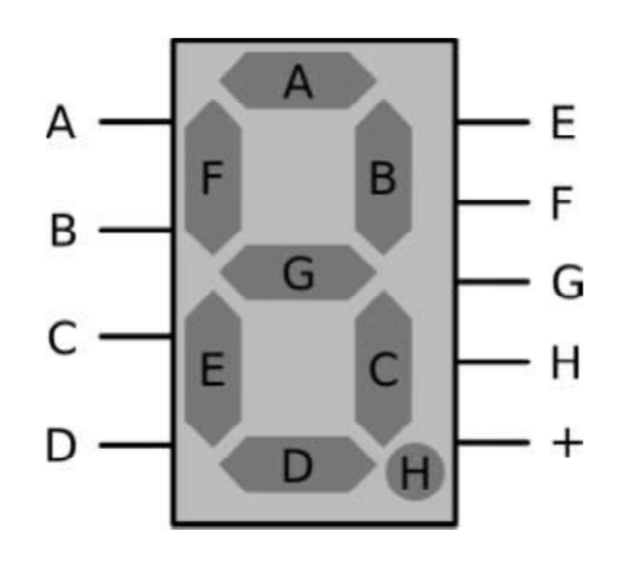
\includegraphics[width=0.5\textwidth]{7segmentdisplay.png}
    \caption{7-Segment Display}
    \label{fig:sevensegdisp}
\end{figure}

\begin{table}[H]
\centering
\begin{tabular}{|c|c|c|c|c|c|c|c|c|}
\hline
\textbf{Value} & \textbf{H} & \textbf{G} & \textbf{F} & \textbf{E} & \textbf{D} & \textbf{C} & \textbf{B} & \textbf{A} \\ \hline
\textbf{0}     & 0          & 0          & 1          & 1          & 1          & 1          & 1          & 1          \\ \hline
\textbf{1}     & 0          & 0          & 0          & 0          & 0          & 1          & 1          & 0          \\ \hline
\textbf{2}     & 0          & 1          & 0          & 1          & 1          & 0          & 1          & 1          \\ \hline
\textbf{3}     & 0          & 1          & 0          & 0          & 1          & 1          & 1          & 1          \\ \hline
\textbf{4}     & 0          & 1          & 1          & 0          & 0          & 1          & 1          & 0          \\ \hline
\textbf{5}     & 0          & 1          & 1          & 0          & 1          & 1          & 0          & 1          \\ \hline
\textbf{6}     & 0          & 1          & 1          & 1          & 1          & 1          & 0          & 1          \\ \hline
\textbf{7}     & 0          & 0          & 0          & 0          & 0          & 1          & 1          & 1          \\ \hline
\textbf{8}     & 0          & 1          & 1          & 1          & 1          & 1          & 1          & 1          \\ \hline
\textbf{9}     & 0          & 1          & 1          & 0          & 1          & 1          & 1          & 1          \\ \hline
\textbf{A}     & 0          & 1          & 1          & 1          & 0          & 1          & 1          & 1          \\ \hline
\textbf{C}     & 0          & 0          & 1          & 1          & 1          & 0          & 0          & 1          \\ \hline
\textbf{E}     & 0          & 1          & 1          & 1          & 1          & 0          & 0          & 1          \\ \hline
\textbf{F}     & 0          & 1          & 1          & 1          & 0          & 0          & 0          & 1          \\ \hline
\textbf{H}     & 0          & 1          & 1          & 1          & 0          & 1          & 1          & 0          \\ \hline
\textbf{I}     & 0          & 0          & 0          & 0          & 0          & 1          & 1          & 0          \\ \hline
\textbf{L}     & 0          & 0          & 1          & 1          & 1          & 0          & 0          & 0          \\ \hline
\textbf{O}     & 0          & 1          & 0          & 1          & 1          & 1          & 0          & 0          \\ \hline
\textbf{P}     & 0          & 1          & 1          & 0          & 1          & 0          & 1          & 1          \\ \hline
\textbf{S}     & 0          & 1          & 1          & 0          & 1          & 1          & 0          & 1          \\ \hline
\textbf{U}     & 0          & 0          & 1          & 1          & 1          & 1          & 1          & 0          \\ \hline
\end{tabular}
\end{table}

\subsection{Part 1}
In the first part of the experiment, a counter program that counts from 0 to 9 repeatedly with 1-second delay at each increment is designed. The numbers are displayed on the 7-segment display.
\newline
In order to implement the desired feature on MSP430, the following piece of
code given in Figure 1 was written.

Line by line explanation is given below.
\begin{itemize}
    \item Line 1-5: These lines include the setup sequence to define functionalities of Port 1 and Port 2. First, all 8 bits of Port 1 and first 4 bits of Port 2 are enabled as outputs. Then all bits of Port 1 is cleared (so no random data will be shown on the display) and first digit of 4-digit 7-segment display is activated on Port 2. Initial value of register R4 that is the memory location for the array arr is assigned.

    \item Line 7-12: This is the main loop. First, the value in R4 is checked to know if the end of the array is reached. If that is the case, program jumps to $Reset_seq$ to go back to the first element in the array. If not, all elements (numbers) in the array show up one by one on Port 1, having 1-second delay each time.
    
    \item Line 16-17: This $Reset_seq$ function sets the arr pointer R4 back to the start of the array arr. It is called when all numbers have been displayed on the screen consecutively. So after each time the number 9 is diplayed, it goes back to 0 again.
    
    \item Line 20-30: This is the Delay function that was already given in lab booklet. It provides the desired 1-second delay.
    
    \item Line 33-34: This is the array arr that holds the bit-wise values that turn on the corresponding LEDs of the 7-segment display in order to display decimal numbers.
\end{itemize}

\begin{figure}[H]
    \centering
    \begin{lstlisting}[language={[x86masm]Assembler}]
Setup		bis.b	#0FFh,		&P1DIR
		bis.b	#00Fh,		&P2DIR
		bic.b	#0FFh,		&P1OUT
		mov.b	#001h,		&P2OUT
		mov.w	#arr, 		r4

Main		cmp	#arr_end, 	r4
		jz	Reset_seq
		mov.b	@r4,		&P1OUT
		call	#Delay
		add	#001h,		r4
		jmp	Main


; Reset sequence
Reset_seq	mov.w	#arr,		r4
		jmp     Main

; Delay function
Delay		push 	r14
		push    r15
		mov.w	#0Ah,		R14
L2		mov.w	#07A00h,	R15
L1		dec.w	R15
		jnz	L1
		dec.w	R14
		jnz	L2
		pop	r15
		pop 	r14
		ret


arr            .byte	00111111b, 00000110b, 01011011b, 01001111b, 01100110b, 01101101b, 01111101b, 00000111b, 01111111b, 01101111b
arr_end
    \end{lstlisting}
    \label{code:part1delay}
    \caption{Code for Part 1}
\end{figure}

%%%%%%%%%%%%%%%%%%%%%%%
\newpage
\subsection{Part 2}
In this part of the experiment an interrupt subroutine that changes the values shown on the display was implemented. The display had two modes:
\begin{itemize}
    \item Writing "Achilles" letter by letter
    \item Showing how many times the word "Achilles" is completed
\end{itemize}
As will be explained later in the code review, 7\textsuperscript{th} button connected to Port 2, was used to initiate the interrupt signal.

\newline{}
In order to implement the aforementioned features on MSP430, the following piece of code given in Figure \ref{code:interrupt_1} and \ref{code:interrupt_2} was written.

\begin{itemize}
    \item Line 1-6: This is the setup sequence to enable interrupt functionality. Port 2's 7\textsuperscript{th} bit is set to 1, enabling interrupt when 7\textsuperscript{th} button is pressed. Remaining bits are set to 0 so I/O functions are selected for corresponding pins. Interrupt flag is set on a high-to-low transition for the 7\textsuperscript{th} bit. Then interrupt flags are cleared and interrupt is enabled for the micro-controller.
    \item Line 8-14: The setup sequence to define functionalities of Ports 1 and 2. First, 8 bits of Port 1 and first 4 bits of Port 2 are enabled as outputs then all bits of Port 1 is cleared (so no random data will be shown on the display) and first digit of 4 digit 7 segment display is activated on Port 2. Initial values of registers R4-R6 are assigned. R4 holds the memory location for the counter array, R5 holds the memory location for the Achilles array -the array that stores bit-wise values to display the characters Achilles in order- and R6 specifies the current mode.
    \item Line 19-26: This is the main loop of the code. First the current mode is checked. If R6 is 1 then the interrupt flag was raised and the count is shown on the display. If R6 is 0 then Achilles is shown on the display. After each delay, the next letter of Achilles is shown until the last letter is reached. In that case the reset sequence for the Achilles array pointer is called.
    \item Line 29-31: This code is executed only when R6 is 1. It shows the value stored in the memory location pointed by R4 on the display. After a second jumps back to main loop and is called again if the user did not change the state.
    \item Line 34-35: Sets the counter array pointer R4 back to the start of the array. It is called when the Achilles is displayed on the screen more than 10 times. So every 10 iterations only the first decimal digit of number of Achilles displayed is shown on the display.
    \item Line 38-42: This is the character reset sequence and it is called when the end of Achilles array is reached. Pointer R5 is set back to the start of the Achilles character array, meanwhile counter array pointer R4 is incremented. If the end of counter array is reached, the pointer is reset back to the start of the array by calling the reset counter array sequence.
    \item Line 44-54: Given delay function that halts the micro-controller for about a second or so.
    \item Line 56-60: The interrupt service routine (ISR). The ISR is called when Port 2 receives an interrupt signal. INT03 interrupt vector is instantiated and the interrupt handler routine in the memory location ISR is called. ISR disables the interrupts and changes the current mode by doing an XOR operation on R6. Then clears the interrupt flag, re-enables the interrupts and returns from interrupt.
    \item Line 62-64: Arrays that hold the bit-wise values that turns on the corresponding LEDs of the 7 segment display for decimal numbers and Achilles characters.
    \item Line 73-74: Interrupt vector for port 2 and the memory location at which the address of the interrupt service routine can be found.
\end{itemize}

\begin{figure}[H]
    \centering
\begin{lstlisting}[language={[x86masm]Assembler}, numbers=left]
setup_INT   bis.b   #040h,      &P2IE
            and.b   #0BFh,      &P2SEL
            and.b   #0BFh,      &P2SEL2
            bis.b   #040h,      &P2IES
            clr     &P2IFG ; Clearing flags
            eint    ;Enabling interrupt

Setup	    bis.b   #0FFh,      &P1DIR
	    mov.b   #00Fh,      &P2DIR
	    bic.b   #0FFh,      &P1OUT
	    mov.b   #001h,      &P2OUT
	    mov.w   #arr,       r4
            mov.w   #ach_arr,   r5
            mov.w   #0000h,     r6
; r4= count_pointer, r5=achilles_pointer, r6=dipslay status
; r6= 0, type achilles
; r6= 1, show count

Main        cmp     #001h,      r6
            jz      Show_count
            mov.b   @r5,        &P1OUT
            call    #Delay
            add     #001h,      r5
            cmp     #ach_end,   r5
            jz      Reset_seq
            jmp     Main

; Display how many times achilles has been written on the screen
Show_count  mov.b   @r4,        &P1OUT
            call    #Delay
            jmp     Main

; Reset count
Reset_count	mov.w	#arr,   r4
		jmp     Main
\end{lstlisting}
    \caption{Interrupt Subroutine Example - Part 1/2}
    \label{code:interrupt_1}
\end{figure}

\begin{figure}[H]
    \centering
\begin{lstlisting}[language={[x86masm]Assembler}, firstnumber=37, numbers=left]
; Reset character sequence
Reset_seq   mov.w   #ach_arr,   r5
            add     #001h,      r4
            cmp     #arr_end,   r4
            jz      Reset_count
            jmp     Main
; Delay function
Delay	    push    r14
	    push    r15
	    mov.w   #0Ah,       R14
L2	    mov.w   #07A00h,    R15
L1	    dec.w   R15
	    jnz     L1
    	    dec.w   R14
	    jnz     L2
    	    pop     r15
    	    pop     r14
    	    ret

ISR         dint
            xor.b   #001h,      r6 ;Changing mode
            clr     &P2IFG
            eint
            reti

arr .byte 00111111b, 00000110b, 01011011b, 01001111b, 01100110b, 01101101b, 01111101b, 00000111b, 01111111b, 01101111b arr_end

ach_arr .byte 01110111b, 00111001b, 01110110b, 00110000b, 00111000b, 00111000b, 01111001b, 01101101b ach_end

; Stack Pointer definition
            .global __STACK_END
            .sect   .stack
            
; Interrupt Vectors
            .sect   ".reset"
            .short  RESET
            .sect   ".int03"
            .short  ISR
\end{lstlisting}
    \caption{Interrupt Subroutine Example - Part 2/2}
    \label{code:interrupt_2}
\end{figure}

\newpage

\section{RESULTS}%conc kısmı niye benim cümlelerim sen kimsin 
In the first part of the experiment an assembly program created that counting 0 to 9 with 1 second delay continiously. Result of the program is observed on the 7 segment-display and everything was smoothly and consistent with our theoretical knowledge.

In the second part of the experiment, letters of "Achilles" are displayed on the 7-segment display with 1 second delay. And how many times the all letters of word "Achilles" are displayed on the 7-segment display are stored on the memory. When pushed Port 2's 7\textsuperscript{th} button interrupt occurred and how many times the word "Achilles" displayed on the 7-segment display are displayed on the 7-segment display. Again pushing to the button the program continues writing letters of "Achilles". 

\section{DISCUSSION}

At the end of the experiment, the importance and role of the ISR were noticed by team members. Also how 7-segment display works and how can be manipulated are learned.

To detect an event, two approach can be applied. Polling and interrupts. If polling approach is applied, all time controlled whether event is occurred. And this is not efficient. If interrupt approach is applied, interrupts let the microprocessor sleep while waiting for the event and when event is occurred handles with that and again sleeps. As a result interrupts are the most efficient way for detecting events. 

There are several issues with this approach. First of all time delays are really hard to maintain since it in inside the main program. Every instruction takes several clock cycles. This results a requirement of recalculating delay time after every change of the program otherwise precision will be lost. In order to prevent this an external interrupt can be applied every second.

In this program we were only able to use one of the digits in 7-segment display which only lets counting up to 10. After completing part-3 we have decided to draw a beautiful picture on the 7-segment display. In order to create the illusion of printing something more than one digit, every digit is lighten up very quickly. 


%Please explain, analyze, and interpret what have you done during the  experiment. 
\newpage
\section{CONCLUSION}
%It was not difficult at all. We just nailed it goddamnit.

With this experiment, team have gained more experience with MSP430 microprocessor. In this experiment, the interrupts the key part of the MSP430 microprocessor are learned. This experiment was the easiest experiment compared to other experiments but the one of the most important experiment. The team has completed this experiment in a very short time. After finishing given tasks, the team has done some experiments on the 7-segment display. Incredible animations are created and it is better understood how the 7 segment display works.



\nocite{overleaf}
\nocite{reportGuide}
\newpage
\addcontentsline{toc}{section}{\numberline {}REFERENCES}

\bibliographystyle{unsrt}
\bibliography{reference}

\end{document}

